\def\year{2019}\relax
\documentclass[letterpaper]{article} % DO NOT CHANGE THIS
\usepackage{aaai19}  % DO NOT CHANGE THIS
\usepackage{times}  % DO NOT CHANGE THIS
\usepackage{helvet} % DO NOT CHANGE THIS
\usepackage{courier}  % DO NOT CHANGE THIS
\usepackage[hyphens]{url}  % DO NOT CHANGE THIS
\usepackage{graphicx} % DO NOT CHANGE THIS
\urlstyle{rm} % DO NOT CHANGE THIS
\def\UrlFont{\rm}  % DO NOT CHANGE THIS
\usepackage{graphicx}  % DO NOT CHANGE THIS
\frenchspacing  % DO NOT CHANGE THIS
\setlength{\pdfpagewidth}{8.5in}  % DO NOT CHANGE THIS
\setlength{\pdfpageheight}{11in}  % DO NOT CHANGE THIS
\nocopyright
\graphicspath{{images/}}
\usepackage{array}
\usepackage{amsmath}
\usepackage{caption,subcaption}
%PDF Info Is REQUIRED.
% For /Author, add all authors within the parentheses, separated by commas. No accents or commands.
% For /Title, add Title in Mixed Case. No accents or commands. Retain the parentheses.
\pdfinfo{
/Title (Image Enhancement Applied to Dynamic Frame Generation)
/Author (Mark Wesley Harris)
} %Leave this	
% /Title ()
% Put your actual complete title (no codes, scripts, shortcuts, or LaTeX commands) within the parentheses in mixed case
% Leave the space between \Title and the beginning parenthesis alone
% /Author ()
% Put your actual complete list of authors (no codes, scripts, shortcuts, or LaTeX commands) within the parentheses in mixed case. 
% Each author should be only by a comma. If the name contains accents, remove them. If there are any LaTeX commands, 
% remove them. 

% DISALLOWED PACKAGES
% \usepackage{authblk} -- This package is specifically forbidden
% \usepackage{balance} -- This package is specifically forbidden
% \usepackage{caption} -- This package is specifically forbidden
% \usepackage{color (if used in text)
% \usepackage{CJK} -- This package is specifically forbidden
% \usepackage{float} -- This package is specifically forbidden
% \usepackage{flushend} -- This package is specifically forbidden
% \usepackage{fontenc} -- This package is specifically forbidden
% \usepackage{fullpage} -- This package is specifically forbidden
% \usepackage{geometry} -- This package is specifically forbidden
% \usepackage{grffile} -- This package is specifically forbidden
% \usepackage{hyperref} -- This package is specifically forbidden
% \usepackage{navigator} -- This package is specifically forbidden
% (or any other package that embeds links such as navigator or hyperref)
% \indentfirst} -- This package is specifically forbidden
% \layout} -- This package is specifically forbidden
% \multicol} -- This package is specifically forbidden
% \nameref} -- This package is specifically forbidden
% \natbib} -- This package is specifically forbidden -- use the following workaround:
% \usepackage{savetrees} -- This package is specifically forbidden
% \usepackage{setspace} -- This package is specifically forbidden
% \usepackage{stfloats} -- This package is specifically forbidden
% \usepackage{tabu} -- This package is specifically forbidden
% \usepackage{titlesec} -- This package is specifically forbidden
% \usepackage{tocbibind} -- This package is specifically forbidden
% \usepackage{ulem} -- This package is specifically forbidden
% \usepackage{wrapfig} -- This package is specifically forbidden
% DISALLOWED COMMANDS
% \nocopyright -- Your paper will not be published if you use this command
% \addtolength -- This command may not be used
% \balance -- This command may not be used
% \baselinestretch -- Your paper will not be published if you use this command
% \clearpage -- No page breaks of any kind may be used for the final version of your paper
% \columnsep -- This command may not be used
% \newpage -- No page breaks of any kind may be used for the final version of your paper
% \pagebreak -- No page breaks of any kind may be used for the final version of your paperr
% \pagestyle -- This command may not be used
% \tiny -- This is not an acceptable font size.
% \vspace{- -- No negative value may be used in proximity of a caption, figure, table, section, subsection, subsubsection, or reference
% \vskip{- -- No negative value may be used to alter spacing above or below a caption, figure, table, section, subsection, subsubsection, or reference

\setcounter{secnumdepth}{0} %May be changed to 1 or 2 if section numbers are desired.

% The file aaai19.sty is the style file for AAAI Press 
% proceedings, working notes, and technical reports.
%
\setlength\titlebox{2.5in} % If your paper contains an overfull \vbox too high warning at the beginning of the document, use this
% command to correct it. You may not alter the value below 2.5 in
\title{Image Enhancement Applied to Dynamic Frame Generation}
%Your title must be in mixed case, not sentence case. 
% That means all verbs (including short verbs like be, is, using,and go), 
% nouns, adverbs, adjectives should be capitalized, including both words in hyphenated terms, while
% articles, conjunctions, and prepositions are lower case unless they
% directly follow a colon or long dash
\author{Mark Wesley Harris\\ % All authors must be in the same font size and format. Use \Large and \textbf to achieve this result when breaking a line
% If you have multiple authors and multiple affiliations
% use superscripts in text and roman font to identify them. For example, Sunil Issar,\textsuperscript{\rm 2} J. Scott Penberthy\textsuperscript{\rm 3} George Ferguson,\textsuperscript{\rm 4} Hans Guesgen\textsuperscript{\rm 5}. Note that the comma should be placed BEFORE the superscript for optimum readability
University of Colorado Colorado Springs\\
wharris2@uccs.edu % email address must be in roman text type, not monospace or sans serif
\And
Jugal Kalita\\
University of Colorado Colorado Springs\\
jkalita@uccs.edu
}
\begin{document}

\maketitle

\begin{abstract}
Image enhancement is
a well-studied problem in Computer Vision.
%a growing topic of interest within the Computer Graphics community.
Since performing detailed enhancements analytically produces poor results,
researchers are now turning to machine learning to solve
this and other complex image processing problems.
Here we attempt to discern the best suited architecture out of the current research available
on image enhacement.
The focus is not only on upscaling, but also on removing noise and other visual artifacts from an input image.
We are thus interested in how networks can learn to remove random anamolies from an image
while retaining clarity.
Two generative models were investigated,
Generative Adversarial Networks and Transformers.
Our evaluation showed that the former improved images with 1.3 times more accuracy on average.
\end{abstract}

\section{Introduction}
Image enhancement is a recent hot-topic in the world of Computer Vision
and Deep Learning. From its many applications to the
fields of surveilence, cinematography, social media, and others,
researchers are currently interested
in finding new ways of improving image resolution and clarity.
Even corporate research and development companies like Google are keen on creating the newest
state-of-the-art image enhancement systems \cite{google}.

Image enhancement involves not only increasing image resolution
(called super-resolution), but also replacing noise and other anomalies with
believable substitutes.
Here we discuss our progress in evaluating
the DCGAN, SRGAN, and Transformer architectures
applied to image enhancement.
We hope the conclusion of this research will
provide a foundation
future advancements in image processing
and Computer Graphics research.

\begin{figure}[htbp]
\centerline{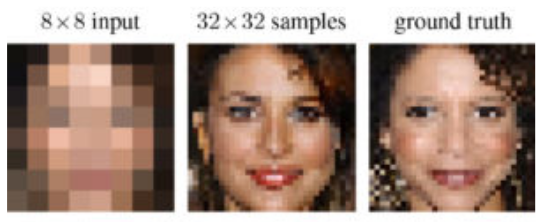
\includegraphics[width=7cm]{google.png}}
\caption{Google \cite{google}.}
\label{fig:google}
\end{figure}

\section{Related Work}
The code developed and evaluated was based off of DCGAN
\cite{generative_adversarial_networks} and SRGAN
\cite{srgan}, and Sparse Attention Transformer
\cite{generative_transformers}.
Basics of each network is discussed below.

\subsection{Generative Adversarial Network}
The Generative Adversarial Network (GAN)
was first proposed as a way to train a model to produce more realistic images
from noise. Essentially the vanilla GAN model works as a random image generator.
The network is made up of two architectures:
a generator, G, and a discriminator, D.
GANs are able to generate new images that have similar qualities to
those in the dataset on which they are trained
\cite{generative_adversarial_networks}.
A generalized GAN architecture is shown in Figure \ref{fig:gan_architecture}.
The model works by training both the generator $G$ and
discriminator $D$ in tandem.

\begin{figure}[htbp]
\centerline{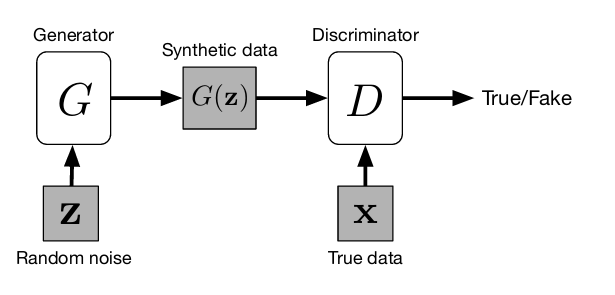
\includegraphics[width=7cm]{gan_architecture.png}}
\caption{Basic Generative Adversarial Network architecture, with a generator $G$
and discriminator $D$
\cite{cgan}.}
\label{fig:gan_architecture}
\end{figure}

$G$ is trained to progressively generate more realistic images,
while $D$ is trained to recognize differences between real and fake inputs.
This relationship can be expressed in the format of a
``two-player min-max game'', shown in Equation \ref{eq:gan_basic}.
Here, $p_{data}(\mathbf{x})$ represents the true data distribution,
and $p_{z}(\mathbf{z})$ represents the distribution of noise.
The goal in training is to minimize the error produced by the generator
and maximize the errors found by the discriminator \cite{cgan}.
Optimizations and variants can be made from this simple concept, of which include
the implementations of cGAN, DCGAN, and SRGAN.

\begin{equation}
\label{eq:gan_basic}
\begin{split}
\text{min}_G\text{max}_DV(D,G) &=
E_{\mathbf{x}\sim p_{data}(\mathbf{x})}[\log D(\mathbf{x})] \\
&+ E_{\mathbf{z}\sim p_{z}(\mathbf{z})}[\log(1 - D(G(\mathbf{z})))]
\end{split}
\end{equation}

\subsection{Transformer}
The Transformer was first proposed
as a way to use attention mechanisms more efficiently.
Attention is a mechanism that references past data during each iteration of training,
in order to discover the complex relationships within the data.
The Transformer relies
``\dots entirely on self-attention to compute representations of its input and output
without using sequence-aligned RNNs or convolution''
\cite{attention_need}.
The Encoder and Decoder for the Transformer design
are shown in Figure \ref{fig:attention}.
An input is first encoded into the dimensional space
the transformer works with,
then the transformed data is processed
and decoded back into a conceivable output.

\begin{figure}[htbp]
\centerline{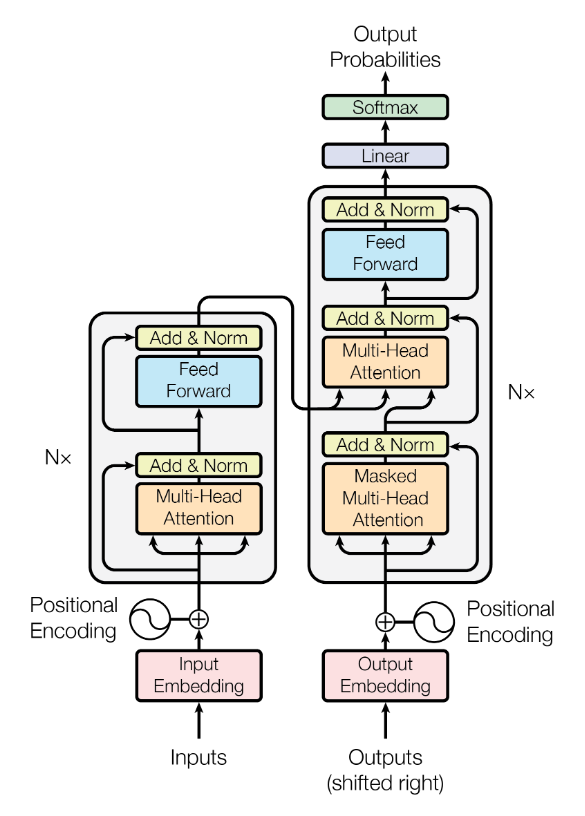
\includegraphics[width=6cm]{attention_architecture.png}}
\caption{Transformer architecture
\cite{attention_need}.}
\label{fig:attention}
\end{figure}

The Transformer uses a series of attention functions to map
between two sequences.
An attention function is a
``\dots mapping [of] a query and a
set of key-value pairs to an output''
\cite{attention_need}.
The mathematical expression of the attention function is shown in
Equation \ref{eq:attention}.
$d_k$ is the dimension of keys and queries, and
$Q,K,V$ are matrices of queries, keys, and values, respectively.
The function uses dotproduct, so that the output is computed as
a weighted sum of the weights
\cite{attention_need}.

\begin{equation}
\label{eq:attention}
\begin{split}
\text{Attention}(Q,K,V) = \text{softmax}(\frac{QK^T}{\sqrt{d_k}})V
\end{split}
\end{equation}

We can model the joint probability of a sequence,
$\mathbf{x}={x_1,x_2,\dots,x_n}$,
as the product of conditional
probability distributions and parameterized by a network $\theta$
\cite{generative_transformers}.
The final expression is shown in Equation \ref{eq:attention_prob}.

\begin{equation}
\label{eq:attention_prob}
p(\mathbf{x}) = \prod_{i=1}^{n}p(x_i|x_1,\dots,x_{i-1};\theta)
\end{equation}

Transformers are able to
``\dots model arbitrary dependencies
in a constant number of layers,''
and are useful for natural language processing and image generation
\cite{generative_transformers}.
While the Transformer shows potential as a powerful machine learning technique,
it is a recent concept and still has many inherent problems.
One of the major problems with the architecture
is that the resources it requires scales with $O(n^2)$
for sequence length $n$. Researchers theorize that
``\dots to improve computational performance for tasks involving very long sequences,
self-attention could be restricted to considering only a neighborhood of size $r$''
\cite{attention_need}.

The Sparse Transformer architecture was developed as a means to shrink the
growth of computational resources for large sequences of data.
Child et al. introduced sparse factorizations on the attention matrix
of a Transformer in order to speed up processing.
An approximation of the dense attention
operation was found by combining several cheaper attention operations.
These optimizations resulted in a faster attention-based architecture
that could be trained on longer sequences of data.

\begin{figure}[htbp]
\centerline{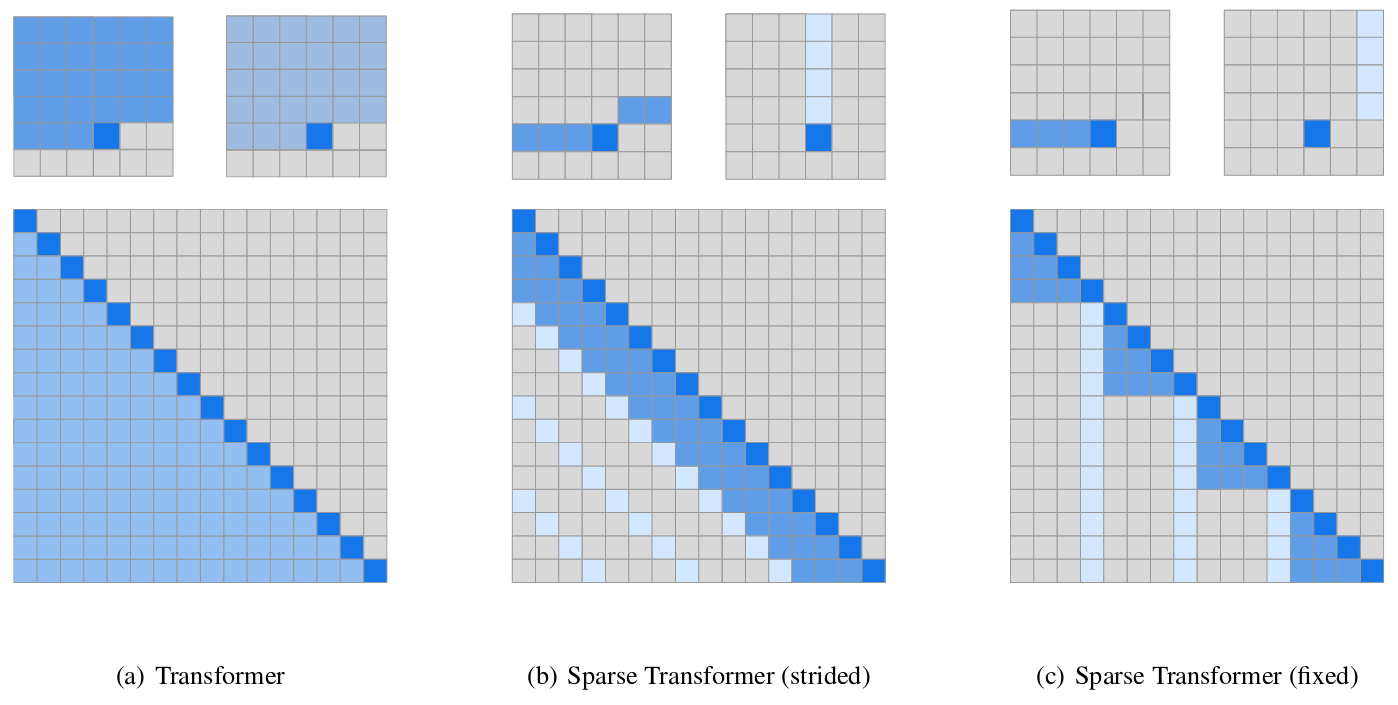
\includegraphics[width=7cm]{attention_comparison.png}}
\caption{Optimizations of Attention
\cite{generative_transformers}.}
\label{fig:attention_optimization}
\end{figure}

Figure \ref{fig:attention_optimization} shows a visual representation of
the two optimizations experimented with, strided and fixed.
The Sparse Attention Transformer architecture reduces the resource cost to
$O(n\sqrt[p]{n})$.
The architecture is also simpler than other autoregressive models that perform
similar functions, including upscaling and enhancement \cite{pixel_subscale}.

\section{Approach}
We now discuss our considerations for the GAN and Transformer implementations.
The first approach studied was the
Deep Convolutional GAN (DCGAN).
The DCGAN
is similar to a regular GAN,
but uses convolutional and convolutional-transpose layers in $D$ and $G$, respectively
\cite{unsupervised_learning}.
Pose Guided Person Image Generation (PG\textsuperscript{2})
proved that a variant conditional DCGAN could be used to
remove anomalies and provide higher resolution for images
\cite{pose_guided_image_generation}.
Without specifics on how the model was altered for image enhancement,
we found it ultimately too difficult to obtain good results from our implementation.
Instead of tuning our imperfect DCGAN, we implemented the
Super Resolution GAN (SRGAN).
The SRGAN was first developed in
Single Image Super Resolution (SISR) research, and showed a drastic decrease in loss measurements
compared to ``NN, bicubic interpolation, and four state-of-the-art methods''
\cite{srgan}.
As opposed to the DCGAN,
the model architecture of the SRGAN was directly applicable to the image enhancement problem,
and did not suffer the same set-backs as we encountered with the DCGAN.
We retain the presumption that the SRGAN architecture could be altered into a better performing DCGAN,
however in order to fully test all architectures we were satisfied with the
initial SRGAN implemented.

Our final implementation was the Sparse Attention Transformer.
Source code for the Transformer was
taken from the Sparse Attention project \cite{generative_transformers}.
The architecture used completely different mechanisims than the GAN models,
requiring a separate runtime environment, Python libraries, and even operating system.
After getting the initial Docker environment set up on a fresh Linux build,
we focused on correctly formulating the tensor inputs of the attention function.
The source code also utilized multi-head attention with a minimum of 4 layers,
which gave us an extra challenge to ensure our inputs were split appropriately to each.

As an overview of the implementations for each architecture,
The DCGAN and SRGAN implementations were written for PyTorch,
while the Transformer architecture used TensorFlow.
A python module of utility functions was created and shared between the programs via GitHub,
so that evaluations of altered images would be consistent and comparable.
A dataset of images was generated
for the purposes of training and testing the developed networks.
The standardized CIFAR-10 dataset
was also used to provide benchmarking and further our analysis.
Each dataset contained approximately 60,000 32 x 32 pixel images.
Random samples are shown in Figure \ref{fig:datasets}.

\subsection{Datasets}
\begin{figure}[h!]
\centering
\begin{subfigure}{0.22\textwidth}
\begin{center}
\begin{minipage}[t]{0.95\linewidth}
\begin{centering}
% FRAME
{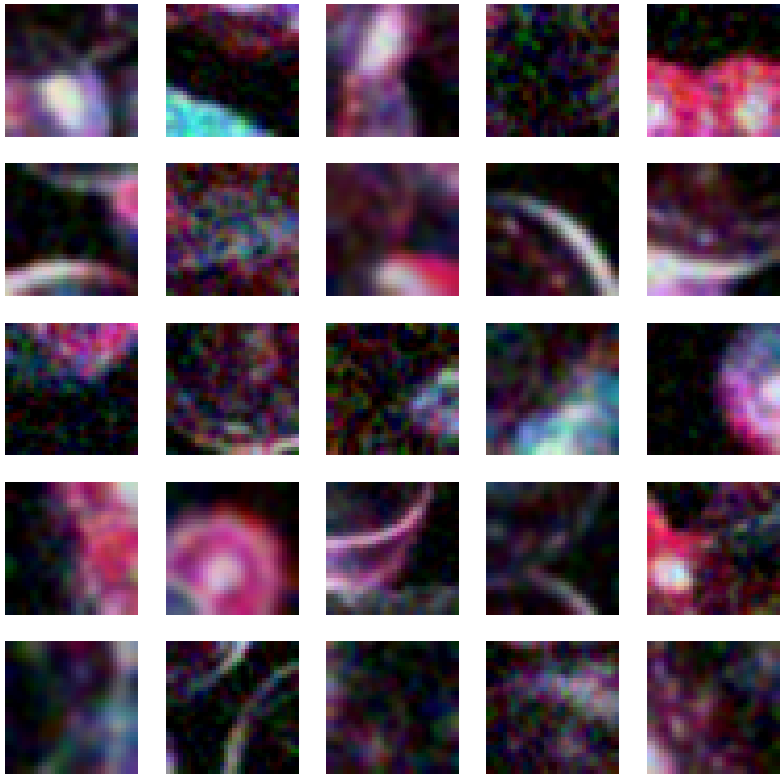
\includegraphics[width=\linewidth]{frame_samplesxrange.png}}
\caption{Generated dataset.}
\label{fig:frame_dataset}
\end{centering}
\end{minipage}
\end{center}
\end{subfigure}
\begin{subfigure}{0.22\textwidth}
\begin{center}
\begin{minipage}[t]{0.95\linewidth}
\begin{centering}
% CIFAR
{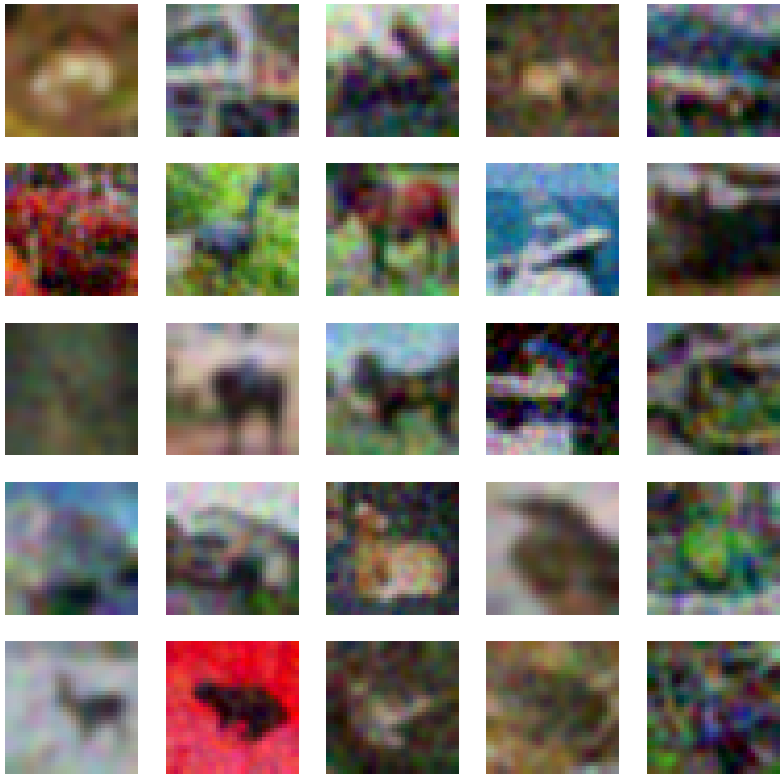
\includegraphics[width=\linewidth]{cifar_samplesxrange.png}}
\caption{CIFAR-10 dataset.}
\label{fig:cifar_dataset}
\end{centering}
\end{minipage}
\end{center}
\end{subfigure}
\caption{Random samples from each dataset evaluated.}
\label{fig:datasets}
\end{figure}

The first dataset evaluated was generated from 300 frames of source animation \cite{animation}.
Each frame was a resolution of 1080 by 1920 pixels.
We refer to the saved images as ``frameblocks'' --
each frameblock was chosen to represent significant change between two source frames.
Frames were processed sequentially, which resulted in a total of 56,337 generated images.
The CIFAR-10 dataset was also used, in order to help evaluate how our models
compare to current research.
The CIFAR-10 data consisted of 10 different categories of images, with 60,000 images total.
Examples of the categories include dogs, horses, frogs, and automobiles.

During training and evaluation, input images from each dataset were pre-processed
in order to produce low resolution versions containing controlled amounts of random anomalies and noise.
Equation \ref{eq:alter} expresses how images were altered to provide the sources for enhancement.
First, a random sample of uniform noise, $I^{N}$, was generated in the shape of
sample image, $I$. A linear combination was applied to add $\alpha$ amount of the input
image with $1 - \alpha$ amount of the random noise
(where $0 \leq \alpha \leq 1$).
Afterwards, a Gaussian blur was applied with scale $\beta$.
We decided to evaluate several different senarios of varying image quality.
The top row of each sample in Figure \ref{fig:example_outputs} shows altered samples
of an image from the CIFAR-10 dataset with varying parameters of $\alpha$ and $\beta$.
The OpenCV Python library was used to perform the same alterations accross all model architectures.

\begin{equation}
\label{eq:alter}
I' = G_{\beta,\beta}(\alpha I + (1 - \alpha)I^{N})
\end{equation}

\subsection{Evaluation}
A major criticism for GANs is the
``lack of a robust and consistent evaluation method\dots''
\cite{gmm}.
As opposed to other machine learning models, GANs do not optimize any kind of objective function,
and operate instead on a learned latent space
which cannot be evaluated analytically.
Thus, in order to evaluate the GAN models,
we must find a way to numerically compare the generated images to their respective targets.

Researchers have defined many different means of comparing two images.
Some of this research is focused on image context, such as if two images have the same
person in them.
This type of analysis would not benefit our project,
since the image needs to be exact --
simply containing similar features is not enough.
Thus, we turned to the measurements of
Mean Squared Error (MSE) and Peak Signal-To-Noise Ratio (PSNR),
since these are both commonly used to evaluate super resolution algorithms
\cite{super_resolution}.
However, since MSE has been found to overlook high-frequency details,
and PSNR involves complicated calculations,
it was decided to not use these methods as a means for evaluation
at this time
\cite{srgan}.

In place of MSE and PSNR, we chose to use the concept of pixel distance
to compare two images.
Pixel distance is often referred to as the $L^2$ distance.
The expression for $L^2$ between two images, $I_1$ and $I_2$, is
shown in Equation \ref{eq:distance} \cite{graphics}.
Here pixels are treated as vectors, and images as
3-dimensional matrices.
For a pixel $\mathbf{P}$,
$\mathbf{P} = \langle r,g,b \rangle$ represents
the red, green, and blue color values,
respectively.
Note that the distance between
two pixels $\mathbf{P}$ and $\mathbf{Q}$ is denoted as
$||\mathbf{P} - \mathbf{Q}|| =
\sqrt{(P_x - Q_x)^2 + (P_y - Q_y)^2 + (P_z - Q_z)^2}$.

\begin{equation}
\label{eq:distance}
\sum_{i=1}^{w \times h}||\mathbf{P_i}^{I_2} - \mathbf{P_i}^{I_1}||
\end{equation}

Each of the 60,000 images in either dataset have resolutions of
32 pixels in width ($w$) and 32 pixels in height ($h$).
Thus, processing a single image pair would consist of summing 1,024
distance calculations.
We found this to be very draining on computational resources --
the square-root operation in particular was problematic.
In order to save time training and evaluating, we chose to replace
traditional $L^2$ distance with a simplification that uses bit-wise XOR.
Since the XOR operation accurately captures differences between color
values without costing much in processing,
we found it to be a credible and efficient replacement of $L^2$ distance
\cite{image_analysis}.
For a visual comparison of standard $L^2$ to our implementation,
see Figure \ref{fig:pixel_distance}.

\begin{equation}
\label{eq:xor}
\sum_{i=1}^{w \times h}\lceil(\sum_{x \in r,g,b}\mathbf{P_i}(x)^{I_2} \oplus \mathbf{P_i}(x)^{I_1})\rceil^{255}
\end{equation}

The XOR calculation used is a much faster image distance calculation than
traditional $L^2$, and represents the same 
The sum of color values ($\sum_{x \in r,g,b}$) is stored in
the corresponding 8-bit pixel of a black and white image.
Values are capped at 255 to avoid erroneous results with overflow.
Percentage of enhancement (e.g. likeness of an image to the target)
is calculated using a ratio of the pixel sum $S_p$
and that of a completely black image, $T_p = 255 \times w \times h$.

\begin{equation}
\label{eq:enhancement}
E = 1 - \frac{S_p}{T_p}
\end{equation}

If the value of image enhancement
is close to 1, then there is very little difference between the generated
image and the target.
Conversely, a value close to 0 implies great difference between the two images.
Visually speaking, a darker image signifies greater difference than a lighter image.

\begin{figure}[h!]
\centering
\begin{subfigure}{0.22\textwidth}
\begin{center}
\begin{minipage}[t]{0.75\linewidth}
\begin{centering}
{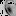
\includegraphics[width=\linewidth]{shadow_standard.png}}
\caption{Example of standard $L^2$ calculation.}
\label{fig:shadow_standard}
\end{centering}
\end{minipage}
\end{center}
\end{subfigure}
\begin{subfigure}{0.22\textwidth}
\begin{center}
\begin{minipage}[t]{0.75\linewidth}
\begin{centering}
{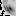
\includegraphics[width=\linewidth]{shadow_ours.png}}
\caption{Example of our distance calculation.}
\label{fig:shadow_ours}
\end{centering}
\end{minipage}
\end{center}
\end{subfigure}
\caption{Visual comparison of pixel distance metrics.}
\label{fig:pixel_distance}
\end{figure}

\section{Challenges}
Since the base DCGAN architecture was created for image generation from noise,
we found no feasible way to inject a conditioning image during training.
Several methods were attempted to fix this problem.
We first attempted to manipulate the Z-latent vector
This is the vector trained by the GAN to map features of one image to another.
Since the latent vector is unknown until training occurs,
it was impractical to initialize it without a way to convert
the condition image into the latent space.
After several attempts, this method was abandoned.

The next approach proved to be more useful than manipulating the latent vector directly.
The GAN was made to generate $G(\mathbf{x})$ of
the expression $I_E = X - G(\mathbf{x})$. The theory behind this approach was to train
the model to generate the enhancement by inversing the alterations made in pre-processing.
The way the generator is setup, however, back-propagation acts on the image generated
and not the calculated image, $I_E$.
Thus, the generator eventually became confused and quickly spiraled out of control thereafter.
When compared to the good results of the SRGAN,
we decided the DCGAN implementation did not provide enough data to support evaluation.
The model does however produce good images from noise,
examples of which are shown in Figure \ref{fig:dcgan_outputs}.

%The Sparse Attention Transformer was the most problematic of all the network architectures we studied.
%The Transformer required a Linux operating system, and the TensorFlow and Blocksparse modules.
%Those two modules required conflicting Python versions, so the only way we could get the source code to run
%was to modify the Blocksparse module scripts and remove Python 3 syntax.
%Despite the misgivings with the architecture, we were able to get it running.
%The next issue we faced was with preparing our image data as inputs into the Transformer.
%We reimagined how to split our data to be fed into the network correctly.

\section{Results}
The SRGAN and Transformer models were trained on 75\% of the dataset, with shuffling,
for each combination of parameters.
The remaining 25\% of images were used for testing.
Green and blue lines are measurements for the CIFAR dataset, while
yellow and red lines are measurements for our generated frameblock dataset.
Means are provided as dashed lines for each distribution.

\begin{figure}[h!]
\centerline{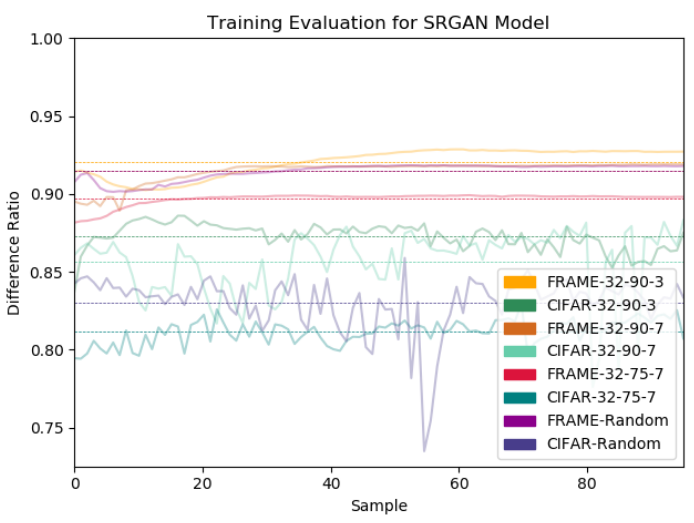
\includegraphics[width=8cm]{srgan_training_results.png}}
\centerline{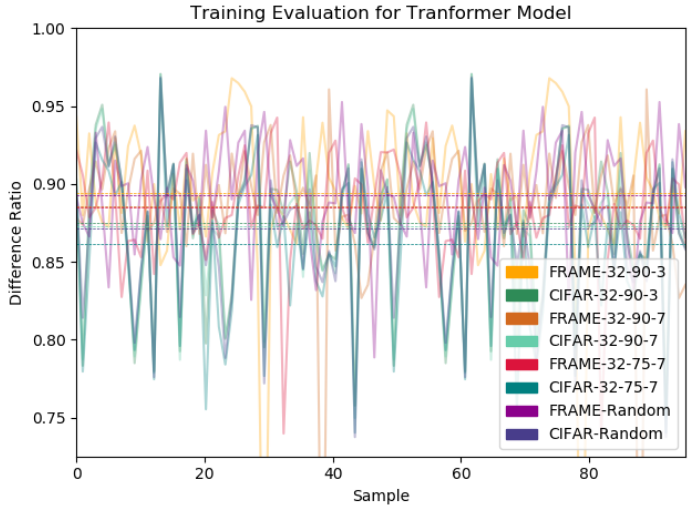
\includegraphics[width=8cm]{attn_training_results.png}}
\caption{Results during training of the SRGAN and Transformer models.}
\label{fig:training_results}
\end{figure}

Figure \ref{fig:training_results} shows the calculated enhancement
during training.
The average enhancement for each distribution is drawn in
a horizontal dashed line.
The results of our tests are presented in Table \ref{tbl:results}.
The SRGAN showed much better trends than the Transformer.
As shown in the graph, we can clearly see that the SRGAN model increased in accuracy over the course of training.
The Transformer's performance was unexpectedly erratic, which explains why some images were over-fit.
The SRGAN model handled each dataset very differently,
and the distinction between to the two distributions is very pronounced.
In comparision, the Transformer seemed to have roughly the same results (both good and bad)
for either dataset. We see the same trend as in the SRGAN on average, however accuracies are much closer together.

As a way of evaluating each model's capabilities for images with unknown amounts of
noise and blurring, we also trained them on images with a range of values.
We were surprised to find that these tests differed only slightly from the least-altered models.
This proves that generative models are appropritate for solving real-world enhancement
problems, where we don't know how much the anamolous data affects a source image.
Overall, our generated dataset performed much better than the CIFAR-10 dataset.
This is what we anticipated, since all images in our dataset had the same qualities --
subject, lighting, color, and negative space were found to influence the model accuracy.

\begin{table}[t]
\begin{centering}
\bgroup
\def\arraystretch{1.5}
\begin{tabular}{| m{0.1025\textwidth} | m{0.0672\textwidth} | m{0.06125\textwidth} | m{0.06125\textwidth} | m{0.06125\textwidth}|} 
\hline
\multicolumn{5}{|c|}{\textbf{Training Evaluation}} \\
\hline
\hline
\textbf{($\boldsymbol{\alpha},\boldsymbol{\beta}$)} & \textbf{(0.75, 7)} & \textbf{(0.9, 7)} & \textbf{(0.9, 3)} & \textbf{Range} \\ 
\hline
\multicolumn{5}{|c|}{\textit{Frame Training Dataset}} \\
\hline
\textbf{SRGAN} & 0.89687 & 0.91459 & 0.92046 & 0.91450 \\
\hline
\textbf{Transformer} & 0.86831 & 0.88479 & 0.89707 & 0.89409 \\
\hline
\multicolumn{5}{|c|}{\textit{CIFAR-10 Training Dataset}} \\
\hline
\textbf{SRGAN} & 0.81159 & 0.85660 & 0.87253 & 0.83036 \\
\hline
\textbf{Transformer} & 0.87515 & 0.87191 & 0.86196 & 0.86804 \\
\hline
\multicolumn{5}{|c|}{\textit{Training Averages}} \\
\hline
\textbf{SRGAN} & 0.85423 & 0.88559 & 0.89649 & 0.87243 \\
\hline
\textbf{Transformer} & 0.87173 & 0.87835 & 0.87951 & 0.88106 \\
\hline
\multicolumn{5}{c}{} \\
\hline
\multicolumn{5}{|c|}{\textbf{Testing Evaluation}} \\
\hline
\hline
\textbf{($\boldsymbol{\alpha},\boldsymbol{\beta}$)} & \textbf{(0.75, 7)} & \textbf{(0.9, 7)} & \textbf{(0.9, 3)} & \textbf{Range} \\ 
\hline
\multicolumn{5}{|c|}{\textit{Frame Testing Dataset}} \\
\hline
\textbf{SRGAN} & 0.84983 & 0.87031 & 0.87105 & 0.85876 \\
\hline
\textbf{Transformer} & 0.65538 & 0.66616 & 0.67249 & 0.66494 \\
\hline
\multicolumn{5}{|c|}{\textit{CIFAR-10 Testing Dataset}} \\
\hline
\textbf{SRGAN} & 0.78727 & 0.83580 & 0.85327 & 0.81697 \\
\hline
\textbf{Transformer} & 0.59138 & 0.59293 & 0.59749 & 0.59504 \\
\hline
\multicolumn{5}{|c|}{\textit{Testing Averages}} \\
\hline
\textbf{SRGAN} & 0.81855 & 0.85305 & 0.86216 & 0.83786 \\
\hline
\textbf{Transformer} & 0.62327 & 0.62960 & 0.63504 & 0.62989 \\
\hline
\end{tabular}
\bigskip
\caption{Evaluation for the SRGAN and Transformer models on each set of parameters.}
\label{tbl:results}
\egroup
\end{centering}
\end{table}

The averages captured in Table \ref{tbl:results} demonstrate the divide between training and testing results.
Both the SRGAN and Transformer suffered a dip in accuracy between training and testing,
however the Transformer's accuracy dropped around 4 times more than the SRGAN.
This result again shows that our Transformer model was over-fitting to some data.
Some final outputs of testing each model are shown in Figure \ref{fig:example_outputs}.
The average SRGAN accuracy on testing data was 0.84291,
while the Transformer had an average accuracy of 0.62945.
This means that the SRGAN was on average 1.3 times as accurate as the Transformer architecture.
Average enhancement for the SRGAN model on testing data was 0.84291,
while average enhancement for the Transformer was 0.62945.

We found that for both models, noise more heavily impacted results than blur.
This effect is demonstrated by the samples shown in Figure \ref{fig:srgan_outputs},
where the most distorted image is not nearly as close to the target image as the enhancements from less noise.
By comparison, the Transformer outputs shown in Figure \ref{rig:attn_outputs}
are much lower quality.
We found this was due to the high variance of the Transformer's accuracy.
Some images were nearly perfect, while others were highly inaccurate.
There was clear a clear trend of over-fitting to certain types of images.
Images of dogs and cars were much clearer than images of horses, for example.
The image we chose as the sample was of median quaility.

\begin{figure}[h!]
\centering
\begin{subfigure}{0.45\textwidth}
\begin{center}
\begin{minipage}[t]{\linewidth}
\begin{centering}
% FRAME
{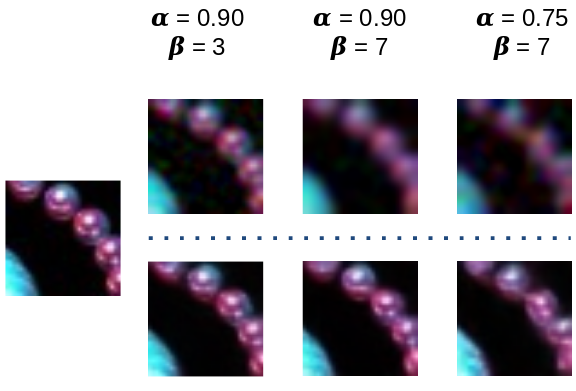
\includegraphics[width=\linewidth]{srgan_outputs.png}}
\caption{SRGAN results on input.}
\label{fig:srgan_outputs}
\end{centering}
\end{minipage}
\end{center}
\end{subfigure}
\begin{subfigure}{0.45\textwidth}
\begin{center}
\begin{minipage}[t]{\linewidth}
\begin{centering}
% CIFAR
{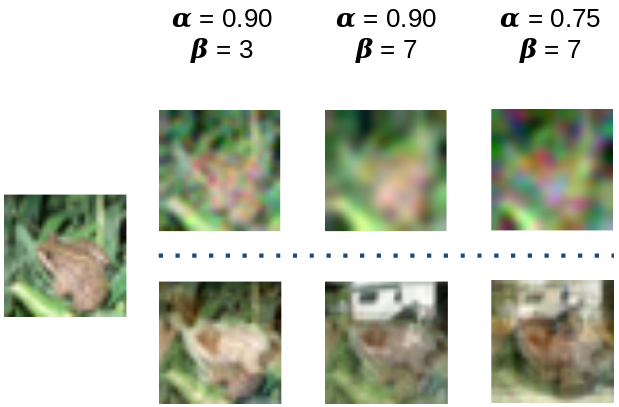
\includegraphics[width=\linewidth]{attn_outputs_2.png}}
\caption{Transformer results on input.}
\label{fig:attn_outputs}
\end{centering}
\end{minipage}
\end{center}
\end{subfigure}
\caption{Example outputs of a single input image for each combination of parameters.}
\label{fig:example_outputs}
\end{figure}

Sample outputs for the DCGAN, SRGAN, Transformer models are
shown in Figures \ref{fig:srgan_outputs}, \ref{fig:attn_outputs}, and \ref{fig:dcgan_outputs}.
The XOR comparison image for each pair of inputs is shown where applicable,
comparing the architecture outputs (left) to real source images (right).

\section{Conclusion}
Image enhancement is a difficult problem to solve.
With the advent of machine learning, however, researchers are now closer
to producing realistic and detailed results.
Here we discussed our work regarding the evaluation of several machine learning architectures.
Our analysis is not exhaustive, there are plenty more models we will
test in the future as applicable. Of these include the
Convolutional Neural Network (CNN) and Conditional GAN (cGAN).

Out of those implemented,
we found that the architecture with the best results was the SRGAN.
While the DCGAN and Transformer models faired poorly in our analysis,
we note that with a few improvements they could conceivably obtain the same results
we saw with the SRGAN.
The added capabilities of Sparse Attention Transformers in particular is also promising
to all image processing problems.
Our work shows how powerful these machine learning models can become.
We look forward to collecting even better results as techologies improve and
lead to new and exciting discoveries.

\begin{figure*}[h!]
\centering
\begin{subfigure}{0.45\textwidth}
\begin{center}
\begin{minipage}[t]{0.95\linewidth}
\begin{centering}
% FRAME
{
\includegraphics[width=0.1\linewidth]{srgan_training_fake_frame_1.png}}
{
\includegraphics[width=0.1\linewidth]{srgan_training_real_frame_1.png}}
{
\includegraphics[width=0.1\linewidth]{srgan_training_shadow_frame_1.png}}
\hfill
{
\includegraphics[width=0.1\linewidth]{srgan_training_fake_frame_2.png}}
{
\includegraphics[width=0.1\linewidth]{srgan_training_real_frame_2.png}}
{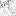
\includegraphics[width=0.1\linewidth]{srgan_training_shadow_frame_2.png}}
\hfill
{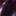
\includegraphics[width=0.1\linewidth]{srgan_training_fake_frame_3.png}}
{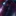
\includegraphics[width=0.1\linewidth]{srgan_training_real_frame_3.png}}
{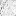
\includegraphics[width=0.1\linewidth]{srgan_training_shadow_frame_3.png}}
\par
{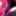
\includegraphics[width=0.1\linewidth]{srgan_training_fake_frame_4.png}}
{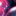
\includegraphics[width=0.1\linewidth]{srgan_training_real_frame_4.png}}
{
\includegraphics[width=0.1\linewidth]{srgan_training_shadow_frame_4.png}}
\hfill
{
\includegraphics[width=0.1\linewidth]{srgan_training_fake_frame_5.png}}
{
\includegraphics[width=0.1\linewidth]{srgan_training_real_frame_5.png}}
{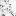
\includegraphics[width=0.1\linewidth]{srgan_training_shadow_frame_5.png}}
\hfill
{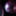
\includegraphics[width=0.1\linewidth]{srgan_training_fake_frame_6.png}}
{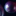
\includegraphics[width=0.1\linewidth]{srgan_training_real_frame_6.png}}
{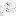
\includegraphics[width=0.1\linewidth]{srgan_training_shadow_frame_6.png}}
\par
{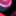
\includegraphics[width=0.1\linewidth]{srgan_training_fake_frame_7.png}}
{
\includegraphics[width=0.1\linewidth]{srgan_training_real_frame_7.png}}
{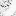
\includegraphics[width=0.1\linewidth]{srgan_training_shadow_frame_7.png}}
\hfill
{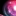
\includegraphics[width=0.1\linewidth]{srgan_training_fake_frame_8.png}}
{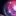
\includegraphics[width=0.1\linewidth]{srgan_training_real_frame_8.png}}
{
\includegraphics[width=0.1\linewidth]{srgan_training_shadow_frame_8.png}}
\hfill
{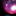
\includegraphics[width=0.1\linewidth]{srgan_training_fake_frame_9.png}}
{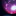
\includegraphics[width=0.1\linewidth]{srgan_training_real_frame_9.png}}
{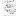
\includegraphics[width=0.1\linewidth]{srgan_training_shadow_frame_9.png}}
% CIFAR
\par\medskip
{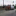
\includegraphics[width=0.1\linewidth]{srgan_training_fake_cifar_1.png}}
{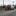
\includegraphics[width=0.1\linewidth]{srgan_training_real_cifar_1.png}}
{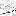
\includegraphics[width=0.1\linewidth]{srgan_training_shadow_cifar_1.png}}
\hfill
{
\includegraphics[width=0.1\linewidth]{srgan_training_fake_cifar_2.png}}
{
\includegraphics[width=0.1\linewidth]{srgan_training_real_cifar_2.png}}
{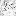
\includegraphics[width=0.1\linewidth]{srgan_training_shadow_cifar_2.png}}
\hfill
{
\includegraphics[width=0.1\linewidth]{srgan_training_fake_cifar_3.png}}
{
\includegraphics[width=0.1\linewidth]{srgan_training_real_cifar_3.png}}
{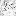
\includegraphics[width=0.1\linewidth]{srgan_training_shadow_cifar_3.png}}
\par
{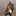
\includegraphics[width=0.1\linewidth]{srgan_training_fake_cifar_4.png}}
{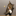
\includegraphics[width=0.1\linewidth]{srgan_training_real_cifar_4.png}}
{\includegraphics[width=0.1\linewidth]{srgan_training_shadow_cifar_4.png}}
\hfill
{\includegraphics[width=0.1\linewidth]{srgan_training_fake_cifar_5.png}}
{\includegraphics[width=0.1\linewidth]{srgan_training_real_cifar_5.png}}
{\includegraphics[width=0.1\linewidth]{srgan_training_shadow_cifar_5.png}}
\hfill
{\includegraphics[width=0.1\linewidth]{srgan_training_fake_cifar_6.png}}
{\includegraphics[width=0.1\linewidth]{srgan_training_real_cifar_6.png}}
{\includegraphics[width=0.1\linewidth]{srgan_training_shadow_cifar_6.png}}
\par
{\includegraphics[width=0.1\linewidth]{srgan_training_fake_cifar_7.png}}
{\includegraphics[width=0.1\linewidth]{srgan_training_real_cifar_7.png}}
{\includegraphics[width=0.1\linewidth]{srgan_training_shadow_cifar_7.png}}
\hfill
{\includegraphics[width=0.1\linewidth]{srgan_training_fake_cifar_8.png}}
{\includegraphics[width=0.1\linewidth]{srgan_training_real_cifar_8.png}}
{\includegraphics[width=0.1\linewidth]{srgan_training_shadow_cifar_8.png}}
\hfill
{\includegraphics[width=0.1\linewidth]{srgan_training_fake_cifar_9.png}}
{\includegraphics[width=0.1\linewidth]{srgan_training_real_cifar_9.png}}
{\includegraphics[width=0.1\linewidth]{srgan_training_shadow_cifar_9.png}}
\caption{SRGAN training results.}
\label{fig:srgan_training_outputs}
\end{centering}
\end{minipage}
\end{center}
\end{subfigure}
\begin{subfigure}{0.45\textwidth}
\begin{center}
\begin{minipage}[t]{0.95\linewidth}
\begin{centering}
% FRAME
{\includegraphics[width=0.1\linewidth]{srgan_testing_fake_frame_1.png}}
{\includegraphics[width=0.1\linewidth]{srgan_testing_real_frame_1.png}}
{\includegraphics[width=0.1\linewidth]{srgan_testing_shadow_frame_1.png}}
\hfill
{\includegraphics[width=0.1\linewidth]{srgan_testing_fake_frame_2.png}}
{\includegraphics[width=0.1\linewidth]{srgan_testing_real_frame_2.png}}
{\includegraphics[width=0.1\linewidth]{srgan_testing_shadow_frame_2.png}}
\hfill
{\includegraphics[width=0.1\linewidth]{srgan_testing_fake_frame_3.png}}
{\includegraphics[width=0.1\linewidth]{srgan_testing_real_frame_3.png}}
{\includegraphics[width=0.1\linewidth]{srgan_testing_shadow_frame_3.png}}
\par
{\includegraphics[width=0.1\linewidth]{srgan_testing_fake_frame_4.png}}
{\includegraphics[width=0.1\linewidth]{srgan_testing_real_frame_4.png}}
{\includegraphics[width=0.1\linewidth]{srgan_testing_shadow_frame_4.png}}
\hfill
{\includegraphics[width=0.1\linewidth]{srgan_testing_fake_frame_5.png}}
{\includegraphics[width=0.1\linewidth]{srgan_testing_real_frame_5.png}}
{\includegraphics[width=0.1\linewidth]{srgan_testing_shadow_frame_5.png}}
\hfill
{\includegraphics[width=0.1\linewidth]{srgan_testing_fake_frame_6.png}}
{\includegraphics[width=0.1\linewidth]{srgan_testing_real_frame_6.png}}
{\includegraphics[width=0.1\linewidth]{srgan_testing_shadow_frame_6.png}}
\par
{\includegraphics[width=0.1\linewidth]{srgan_testing_fake_frame_7.png}}
{\includegraphics[width=0.1\linewidth]{srgan_testing_real_frame_7.png}}
{\includegraphics[width=0.1\linewidth]{srgan_testing_shadow_frame_7.png}}
\hfill
{\includegraphics[width=0.1\linewidth]{srgan_testing_fake_frame_8.png}}
{\includegraphics[width=0.1\linewidth]{srgan_testing_real_frame_8.png}}
{\includegraphics[width=0.1\linewidth]{srgan_testing_shadow_frame_8.png}}
\hfill
{\includegraphics[width=0.1\linewidth]{srgan_testing_fake_frame_9.png}}
{\includegraphics[width=0.1\linewidth]{srgan_testing_real_frame_9.png}}
{\includegraphics[width=0.1\linewidth]{srgan_testing_shadow_frame_9.png}}
% CIFAR
\par\medskip
{\includegraphics[width=0.1\linewidth]{srgan_testing_fake_cifar_1.png}}
{\includegraphics[width=0.1\linewidth]{srgan_testing_real_cifar_1.png}}
{\includegraphics[width=0.1\linewidth]{srgan_testing_shadow_cifar_1.png}}
\hfill
{\includegraphics[width=0.1\linewidth]{srgan_testing_fake_cifar_2.png}}
{\includegraphics[width=0.1\linewidth]{srgan_testing_real_cifar_2.png}}
{\includegraphics[width=0.1\linewidth]{srgan_testing_shadow_cifar_2.png}}
\hfill
{\includegraphics[width=0.1\linewidth]{srgan_testing_fake_cifar_3.png}}
{\includegraphics[width=0.1\linewidth]{srgan_testing_real_cifar_3.png}}
{\includegraphics[width=0.1\linewidth]{srgan_testing_shadow_cifar_3.png}}
\par
{\includegraphics[width=0.1\linewidth]{srgan_testing_fake_cifar_4.png}}
{\includegraphics[width=0.1\linewidth]{srgan_testing_real_cifar_4.png}}
{\includegraphics[width=0.1\linewidth]{srgan_testing_shadow_cifar_4.png}}
\hfill
{\includegraphics[width=0.1\linewidth]{srgan_testing_fake_cifar_5.png}}
{\includegraphics[width=0.1\linewidth]{srgan_testing_real_cifar_5.png}}
{\includegraphics[width=0.1\linewidth]{srgan_testing_shadow_cifar_5.png}}
\hfill
{\includegraphics[width=0.1\linewidth]{srgan_testing_fake_cifar_6.png}}
{\includegraphics[width=0.1\linewidth]{srgan_testing_real_cifar_6.png}}
{\includegraphics[width=0.1\linewidth]{srgan_testing_shadow_cifar_6.png}}
\par
{\includegraphics[width=0.1\linewidth]{srgan_testing_fake_cifar_7.png}}
{\includegraphics[width=0.1\linewidth]{srgan_testing_real_cifar_7.png}}
{\includegraphics[width=0.1\linewidth]{srgan_testing_shadow_cifar_7.png}}
\hfill
{\includegraphics[width=0.1\linewidth]{srgan_testing_fake_cifar_8.png}}
{\includegraphics[width=0.1\linewidth]{srgan_testing_real_cifar_8.png}}
{\includegraphics[width=0.1\linewidth]{srgan_testing_shadow_cifar_8.png}}
\hfill
{\includegraphics[width=0.1\linewidth]{srgan_testing_fake_cifar_9.png}}
{\includegraphics[width=0.1\linewidth]{srgan_testing_real_cifar_9.png}}
{\includegraphics[width=0.1\linewidth]{srgan_testing_shadow_cifar_9.png}}
\caption{SRGAN testing results.}
\label{fig:srgan_testing_outputs}
\end{centering}
\end{minipage}
\end{center}
\end{subfigure}
\caption{Super Resolution GAN evaluation.}
\label{fig:srgan_outputs}
\end{figure*}

\begin{figure*}[h!]
\centering
\begin{subfigure}{0.45\textwidth}
\begin{center}
\begin{minipage}[t]{0.95\linewidth}
\begin{centering}
% FRAME
{\includegraphics[width=0.1\linewidth]{attn_training_fake_frame_1.png}}
{\includegraphics[width=0.1\linewidth]{attn_training_real_frame_1.png}}
{\includegraphics[width=0.1\linewidth]{attn_training_shadow_frame_1.png}}
\hfill
{\includegraphics[width=0.1\linewidth]{attn_training_fake_frame_2.png}}
{\includegraphics[width=0.1\linewidth]{attn_training_real_frame_2.png}}
{\includegraphics[width=0.1\linewidth]{attn_training_shadow_frame_2.png}}
\hfill
{\includegraphics[width=0.1\linewidth]{attn_training_fake_frame_3.png}}
{\includegraphics[width=0.1\linewidth]{attn_training_real_frame_3.png}}
{\includegraphics[width=0.1\linewidth]{attn_training_shadow_frame_3.png}}
\par
{\includegraphics[width=0.1\linewidth]{attn_training_fake_frame_4.png}}
{\includegraphics[width=0.1\linewidth]{attn_training_real_frame_4.png}}
{\includegraphics[width=0.1\linewidth]{attn_training_shadow_frame_4.png}}
\hfill
{\includegraphics[width=0.1\linewidth]{attn_training_fake_frame_5.png}}
{\includegraphics[width=0.1\linewidth]{attn_training_real_frame_5.png}}
{\includegraphics[width=0.1\linewidth]{attn_training_shadow_frame_5.png}}
\hfill
{\includegraphics[width=0.1\linewidth]{attn_training_fake_frame_6.png}}
{\includegraphics[width=0.1\linewidth]{attn_training_real_frame_6.png}}
{\includegraphics[width=0.1\linewidth]{attn_training_shadow_frame_6.png}}
\par
{\includegraphics[width=0.1\linewidth]{attn_training_fake_frame_7.png}}
{\includegraphics[width=0.1\linewidth]{attn_training_real_frame_7.png}}
{\includegraphics[width=0.1\linewidth]{attn_training_shadow_frame_7.png}}
\hfill
{\includegraphics[width=0.1\linewidth]{attn_training_fake_frame_8.png}}
{\includegraphics[width=0.1\linewidth]{attn_training_real_frame_8.png}}
{\includegraphics[width=0.1\linewidth]{attn_training_shadow_frame_8.png}}
\hfill
{\includegraphics[width=0.1\linewidth]{attn_training_fake_frame_9.png}}
{\includegraphics[width=0.1\linewidth]{attn_training_real_frame_9.png}}
{\includegraphics[width=0.1\linewidth]{attn_training_shadow_frame_9.png}}
% CIFAR
\par\medskip
{\includegraphics[width=0.1\linewidth]{attn_training_fake_cifar_1.png}}
{\includegraphics[width=0.1\linewidth]{attn_training_real_cifar_1.png}}
{\includegraphics[width=0.1\linewidth]{attn_training_shadow_cifar_1.png}}
\hfill
{\includegraphics[width=0.1\linewidth]{attn_training_fake_cifar_2.png}}
{\includegraphics[width=0.1\linewidth]{attn_training_real_cifar_2.png}}
{\includegraphics[width=0.1\linewidth]{attn_training_shadow_cifar_2.png}}
\hfill
{\includegraphics[width=0.1\linewidth]{attn_training_fake_cifar_3.png}}
{\includegraphics[width=0.1\linewidth]{attn_training_real_cifar_3.png}}
{\includegraphics[width=0.1\linewidth]{attn_training_shadow_cifar_3.png}}
\par
{\includegraphics[width=0.1\linewidth]{attn_training_fake_cifar_4.png}}
{\includegraphics[width=0.1\linewidth]{attn_training_real_cifar_4.png}}
{\includegraphics[width=0.1\linewidth]{attn_training_shadow_cifar_4.png}}
\hfill
{\includegraphics[width=0.1\linewidth]{attn_training_fake_cifar_5.png}}
{\includegraphics[width=0.1\linewidth]{attn_training_real_cifar_5.png}}
{\includegraphics[width=0.1\linewidth]{attn_training_shadow_cifar_5.png}}
\hfill
{\includegraphics[width=0.1\linewidth]{attn_training_fake_cifar_6.png}}
{\includegraphics[width=0.1\linewidth]{attn_training_real_cifar_6.png}}
{\includegraphics[width=0.1\linewidth]{attn_training_shadow_cifar_6.png}}
\par
{\includegraphics[width=0.1\linewidth]{attn_training_fake_cifar_7.png}}
{\includegraphics[width=0.1\linewidth]{attn_training_real_cifar_7.png}}
{\includegraphics[width=0.1\linewidth]{attn_training_shadow_cifar_7.png}}
\hfill
{\includegraphics[width=0.1\linewidth]{attn_training_fake_cifar_8.png}}
{\includegraphics[width=0.1\linewidth]{attn_training_real_cifar_8.png}}
{\includegraphics[width=0.1\linewidth]{attn_training_shadow_cifar_8.png}}
\hfill
{\includegraphics[width=0.1\linewidth]{attn_training_fake_cifar_9.png}}
{\includegraphics[width=0.1\linewidth]{attn_training_real_cifar_9.png}}
{\includegraphics[width=0.1\linewidth]{attn_training_shadow_cifar_9.png}}
\caption{Transformer training results.}
\label{fig:attn_training_outputs}
\end{centering}
\end{minipage}
\end{center}
\end{subfigure}
\begin{subfigure}{0.45\textwidth}
\begin{center}
\begin{minipage}[t]{0.95\linewidth}
\begin{centering}
% FRAME
{\includegraphics[width=0.1\linewidth]{attn_testing_fake_frame_1.png}}
{\includegraphics[width=0.1\linewidth]{attn_testing_real_frame_1.png}}
{\includegraphics[width=0.1\linewidth]{attn_testing_shadow_frame_1.png}}
\hfill
{\includegraphics[width=0.1\linewidth]{attn_testing_fake_frame_2.png}}
{\includegraphics[width=0.1\linewidth]{attn_testing_real_frame_2.png}}
{\includegraphics[width=0.1\linewidth]{attn_testing_shadow_frame_2.png}}
\hfill
{\includegraphics[width=0.1\linewidth]{attn_testing_fake_frame_3.png}}
{\includegraphics[width=0.1\linewidth]{attn_testing_real_frame_3.png}}
{\includegraphics[width=0.1\linewidth]{attn_testing_shadow_frame_3.png}}
\par
{\includegraphics[width=0.1\linewidth]{attn_testing_fake_frame_4.png}}
{\includegraphics[width=0.1\linewidth]{attn_testing_real_frame_4.png}}
{\includegraphics[width=0.1\linewidth]{attn_testing_shadow_frame_4.png}}
\hfill
{\includegraphics[width=0.1\linewidth]{attn_testing_fake_frame_5.png}}
{\includegraphics[width=0.1\linewidth]{attn_testing_real_frame_5.png}}
{\includegraphics[width=0.1\linewidth]{attn_testing_shadow_frame_5.png}}
\hfill
{\includegraphics[width=0.1\linewidth]{attn_testing_fake_frame_6.png}}
{\includegraphics[width=0.1\linewidth]{attn_testing_real_frame_6.png}}
{\includegraphics[width=0.1\linewidth]{attn_testing_shadow_frame_6.png}}
\par
{\includegraphics[width=0.1\linewidth]{attn_testing_fake_frame_7.png}}
{\includegraphics[width=0.1\linewidth]{attn_testing_real_frame_7.png}}
{\includegraphics[width=0.1\linewidth]{attn_testing_shadow_frame_7.png}}
\hfill
{\includegraphics[width=0.1\linewidth]{attn_testing_fake_frame_8.png}}
{\includegraphics[width=0.1\linewidth]{attn_testing_real_frame_8.png}}
{\includegraphics[width=0.1\linewidth]{attn_testing_shadow_frame_8.png}}
\hfill
{\includegraphics[width=0.1\linewidth]{attn_testing_fake_frame_9.png}}
{\includegraphics[width=0.1\linewidth]{attn_testing_real_frame_9.png}}
{\includegraphics[width=0.1\linewidth]{attn_testing_shadow_frame_9.png}}
% CIFAR
\par\medskip
{\includegraphics[width=0.1\linewidth]{attn_testing_fake_cifar_1.png}}
{\includegraphics[width=0.1\linewidth]{attn_testing_real_cifar_1.png}}
{\includegraphics[width=0.1\linewidth]{attn_testing_shadow_cifar_1.png}}
\hfill
{\includegraphics[width=0.1\linewidth]{attn_testing_fake_cifar_2.png}}
{\includegraphics[width=0.1\linewidth]{attn_testing_real_cifar_2.png}}
{\includegraphics[width=0.1\linewidth]{attn_testing_shadow_cifar_2.png}}
\hfill
{\includegraphics[width=0.1\linewidth]{attn_testing_fake_cifar_3.png}}
{\includegraphics[width=0.1\linewidth]{attn_testing_real_cifar_3.png}}
{\includegraphics[width=0.1\linewidth]{attn_testing_shadow_cifar_3.png}}
\par
{\includegraphics[width=0.1\linewidth]{attn_testing_fake_cifar_4.png}}
{\includegraphics[width=0.1\linewidth]{attn_testing_real_cifar_4.png}}
{\includegraphics[width=0.1\linewidth]{attn_testing_shadow_cifar_4.png}}
\hfill
{\includegraphics[width=0.1\linewidth]{attn_testing_fake_cifar_5.png}}
{\includegraphics[width=0.1\linewidth]{attn_testing_real_cifar_5.png}}
{\includegraphics[width=0.1\linewidth]{attn_testing_shadow_cifar_5.png}}
\hfill
{\includegraphics[width=0.1\linewidth]{attn_testing_fake_cifar_6.png}}
{\includegraphics[width=0.1\linewidth]{attn_testing_real_cifar_6.png}}
{\includegraphics[width=0.1\linewidth]{attn_testing_shadow_cifar_6.png}}
\par
{\includegraphics[width=0.1\linewidth]{attn_testing_fake_cifar_7.png}}
{\includegraphics[width=0.1\linewidth]{attn_testing_real_cifar_7.png}}
{\includegraphics[width=0.1\linewidth]{attn_testing_shadow_cifar_7.png}}
\hfill
{\includegraphics[width=0.1\linewidth]{attn_testing_fake_cifar_8.png}}
{\includegraphics[width=0.1\linewidth]{attn_testing_real_cifar_8.png}}
{\includegraphics[width=0.1\linewidth]{attn_testing_shadow_cifar_8.png}}
\hfill
{\includegraphics[width=0.1\linewidth]{attn_testing_fake_cifar_9.png}}
{\includegraphics[width=0.1\linewidth]{attn_testing_real_cifar_9.png}}
{\includegraphics[width=0.1\linewidth]{attn_testing_shadow_cifar_9.png}}
\caption{Transformer testing results.}
\label{fig:attn_testing_outputs}
\end{centering}
\end{minipage}
\end{center}
\end{subfigure}
\caption{Generative Sparse Transformer evaluation.}
\label{fig:attn_outputs}
\end{figure*}

\begin{figure*}[h!]
\centering
\begin{subfigure}{0.45\textwidth}
\begin{center}
\begin{minipage}[t]{0.95\linewidth}
\begin{centering}
% FRAME
{\includegraphics[width=\linewidth]{dcgan_real.png}}
\caption{DCGAN real samples.}
\label{fig:dcgan_source}
\end{centering}
\end{minipage}
\end{center}
\end{subfigure}
\begin{subfigure}{0.45\textwidth}
\begin{center}
\begin{minipage}[t]{0.95\linewidth}
\begin{centering}
% CIFAR
{\includegraphics[width=\linewidth]{dcgan_fake.png}}
\caption{DCGAN generated samples.}
\label{fig:dcgan_generated}
\end{centering}
\end{minipage}
\end{center}
\end{subfigure}
\caption{Deep Convolutional GAN evaluation.}
\label{fig:dcgan_outputs}
\end{figure*}

\nocite{overview}

\bibliography{final}
\bibliographystyle{aaai}

\end{document}
